\begin{figure}
	\centering
	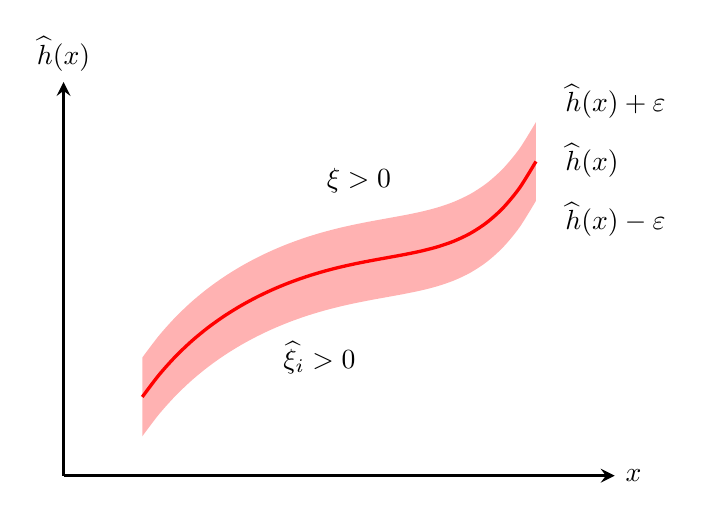
\begin{tikzpicture}
    
		\draw[very thick,-stealth] (0,0) -- (7,0) node[right] {$x$};
		\draw[very thick,-stealth] (0,0) -- (0,5) node[above] {$\widehat{h}(x)$};

		\fill[red!30] (1,0.5) -- ++(0,1) --  plot[domain=1:6,smooth,variable=\x] ({\x},{0.00416667*\x^5-0.0625*\x^4+0.395833*\x^3-1.4375*\x^2+3.35*\x-0.75})
			-- ++(0,-1) -- plot[domain=6:1,smooth,variable=\x] ({\x},{0.00416667*\x^5-0.0625*\x^4+0.395833*\x^3-1.4375*\x^2+3.35*\x-1.75}) -- cycle;

		\draw[domain=1:6,smooth,variable=\x,red,very thick] plot ({\x},{0.00416667*\x^5-0.0625*\x^4+0.395833*\x^3-1.4375*\x^2+3.35*\x-1.25});

		\node[anchor=west] at (6.25,4) {$\widehat{h}(x)$};
		\node[anchor=west] at (6.25,4.75) {$\widehat{h}(x) + \varepsilon$};
		\node[anchor=west] at (6.25,3.25) {$\widehat{h}(x) - \varepsilon$};

		\node at (3.75,3.75) {$\xi > 0$};
		\node at (3.25,1.5) {$\widehat{\xi}_i > 0$};
		
	\end{tikzpicture}
\end{figure}